% now lets talk about the section that compares prior methods and CQL with function approximation in terms of action gap
%%SL.5.11: I wonder if it could make sense to have a single "Related Work and Connections to Policy Constraints" section, where we could have a subsection on "Related Prior Work" subsection on "Prior Work on Offline RL with Constraints" and "Comparative Analysis of CQL and Policy Constraint Methods" or something? Not certain about this, but maybe we try it and see how it looks? It's a bit unconventional...

% setup the stage, what we want to do in this section and why
In this section, we discuss in detail the consequences of the gap-expanding behavior of CQL backups over prior methods based on policy constraints that, as we show in this section, may not exhibit such gap-expanding behavior in practice. To recap, Theorem~\ref{thm:gap_amplify} shows that the CQL backup operator increases the difference between expected Q-value at in-distribution ($\mathbf{a} \sim \behavior(\mathbf{a}|\bs)$) and out-of-distribution ($\mathbf{a} \text{~s.t.~} \frac{\mu_k(\mathbf{a}|\bs)}{\behavior(\mathbf{a}|\bs)} << 1$) actions. We refer to this property as the gap-expanding property of the CQL update operator.

% This gap-expanding behavior plays a central role when learning in the presence of function approximation:  

% In this section, we perform an analysis of CQL with deep neural networks, and compare it to prior offline RL methods based on policy constraints. As noted in Section~\ref{sec:related}, some variants of CQL can be viewed as applying a policy constraint on the greedy policy induced by the Q-function. We therefore aim to analyze the effect of direct regularization on the Q-function as opposed to only constraining the policy, with primary focus on settings where function approximation is employed.

% discuss why policy constraint methods may fail
\textbf{Function approximation may give rise to erroneous Q-values at OOD actions.} We start by discussing the behavior of prior methods based on policy constraints~\citep{kumar2019stabilizing,fujimoto2018off,jaques2019way,wu2019behavior} in the presence of function approximation.
To recap, because computing the target value requires $\E_\policy[\hat{Q}(\bs,\mathbf{a})]$, constraining $\policy$ to be close to $\behavior$ will avoid evaluating $\hat{Q}$ on OOD actions. These methods typically do not impose any further form of regularization on the learned Q-function.
Even with policy constraints, because function approximation used to represent the Q-function, learned Q-values at two distinct state-action pairs are coupled together. As prior work has argued and shown~\citep{achiam2019towards,fu2019diagnosing,kumar2020discor}, the ``generalization'' or the coupling effects of the function approximator may be heavily influenced by the properties of the data distribution~\citep{fu2019diagnosing,kumar2020discor}. For instance, \citet{fu2019diagnosing} empirically shows that when the dataset distribution is narrow (i.e. state-action marginal entropy, $\mathcal{H}(d^\behavior(\bs, \mathbf{a}))$, is low~\citep{fu2019diagnosing}), the coupling effects of the Q-function approximator can give rise to incorrect Q-values at different states, though this behavior is absent without function approximation, and is not as severe with high-entropy (e.g. Uniform) state-action marginal distributions.
%%SL.5.27: The above sentence is really speculative -- I don't think it's at all clear why narrow datasets couple different state action pairs. It's also very hard to understand, because it's long, with multiple clauses, and nested parentheses. I would really recommend just deleting the whole sentence. But if you don't want to delete it, try to rewrite to more clearly explain the point, with shorter sentences, avoiding complex clauses, and avoiding parens whenever possible.
% done, cited prior work diagnosing bottlenecks and DisCor

In offline RL, we will shortly present empirical evidence on high-dimensional MuJoCo tasks showing that certain dataset distributions, $\mathcal{D}$, may cause the learned Q-value at an OOD action $\mathbf{a}$ at a state $\bs$, to in fact take on high values than Q-values at in-distribution actions at intermediate iterations of learning. This problem persists even when a large number of samples (e.g. $1M$) are provided for training, and the agent cannot correct these errors due to no active data collection.  

%%AK.5.29: Toned down to one para, with mostly pointing to the analysis, not creating any hypotheses for why something might be going wrong.
Since actor-critic methods, including those with policy constraints, use the learned Q-function to train the policy, in an iterative online policy evaluation and policy improvement cycle, as discussed in Section~\ref{sec:background}, the errneous Q-function may push the policy towards OOD actions, especially when no policy constraints are used. Of course, policy constraints should prevent the policy from choosing OOD actions, however, as we will show that in certain cases, policy constraint methods might also fail to prevent the effects on the policy due to incorrectly high Q-values at OOD actions. 

% how do these Q-values affect the policy?
% \textbf{How can erroneous Q-values affect the quality of the resulting policy?} When these erroneous Q-values -- with higher relative values
% at out-of-distribution actions -- are used to then update the policy, the policy is pushed towards OOD actions, since a policy improvement update, shown below, trains the policy to maximize Q-values:
% \begin{equation}
%     \label{eqn:policy_constraint_repeated}
%     \policy^{k+1}~~ \leftarrow \arg \max_{\textcolor{red}{\policy}} \E_{\bs \sim d^\behavior(\bs)}\left[ \E_{\mathbf{a} \sim \textcolor{red}{\policy}}[\hat{Q}^{k+1}(\bs, \mathbf{a})] - \nu_k \underbrace{D(\textcolor{red}{\policy}(\mathbf{a}|\bs), \behavior(\mathbf{a}|\bs))}_{\text{policy constraint}} \right]
% \end{equation}
% % Of course, when policy constraints are used, the policy is prevented from choosing OOD actions. 
% % However, a gradient signal obtained from such an erroneous Q-function will still push the policy towards OOD actions, since the Q-values at these OOD actions are relatively higher than in-distribution actions. We discuss empirical evidence justifying this in Appendix~\ref{app:empirical_evidence_gap_expanding}. 
% %%SL.5.27: A reviewer might say this should not be an issue, since you won't get OOD actions due to the constraint
% % We have empirical evidence for this, that atleast in some cases this could be an issue, but the example, and the experiments, I feel should justify this in practice
% However, the low fidelity of the Q-function combined with the inability to correct errors in the function this case, may just push the policy towards OOD actions, directly conflicting with the policy-constraint. While this might not be potentially harmful when the Q-function provides enough improvement signal to improve the policy when the policy constraint is satisfied, but this property may not be guaranteed. 

% As a result, the improvement signal obtained from the Q-function might directly conflicts with the policy constraint, whose role is to prevent the policy from choosing OOD actions. We would instead desire that the Q-function provides enough improvement signal to the policy within the space of in-distribution actions, so that the policy can improve within the set of observed actions. But since Q-values may be higher at OOD actions, the Q-function gradient may push the policy towards OOD actions as a result, and hence directly conflict with the policy constraint (which aims at keeping the policy within in a close neighbourhood of the behavior cloned policy).  
% When gradient based optimization is used to train the policy in this setting, this could amount to conflicting gradient (as we show via empirical evidence), and hence, it is likely that the overall update shown in Equation~\ref{eqn:policy_constraint_repeated} does not improve the policy meaningfully. 
%%SL.5.27: this seems very vague and imprecise, and it's not clear how CQL does this
% restated below

\textbf{How can CQL address this problem?} As we show in Theorem~\ref{thm:gap_amplify}, the difference between expected Q-values at in-distribution actions and out-of-distribution actions is expanded by the CQL update. This property is a direct consequence of the specific nature of the CQL regularizer -- that maximizes Q-values under the dataset distribution, and minimizes them otherwise. This difference depends upon the choice of $\alpha_k$, which can directly be controlled, since it is a free parameter. Thus, by effectively controlling $\alpha_k$, CQL can push down the learned Q-value at out-of-distribution actions as much is desired, correcting for the erroneous overestimation error in the process.  


%%SL.5.27: Overall, I really don't find the discussion above to be very convincing. It seems very speculative, and it's very easy to argue with and disagree with. Are you sure we can't somehow delete the stuff above, and instead present this appendix as a summary of the evidence that we'll be discussing below? I also think we should really consider simply deleting this appendix. It was a nice idea, but the quality of the evidence here is really not up to the standard of rigor, and perhaps it's better to omit it than to include things that are too debatable or too hand-wavy. Basically, I have a hard time imagining how this appendix will make anyone happy -- anyone who is skeptical about our method will become even more skeptical, whereas anyone who likely our method will probably not read this appendix (because it's not about our method).

% why is this problem more relevant in offline settings?
% We also remark that while the problem induced due to Q-function approximation also afflicts standard online Q-function training (and this is a motivation behind gap-increasing operators~\citep{bellemare2016increasing}), we would expect this problem to more severely affect performance in offline RL. Q-function errors in standard online RL can be corrected in most cases~\citep{kumar2020discor,levine2020offline}, since the agent can collect new transitions that correspond to highly erroneous Q-values and then train on them. However, the algorithm cannot perform any online data collection and moreover, has no control over the dataset, $\mathcal{D}$ either in offline RL settings, making the impact of this problem severe. We next present a simple didactic example to demonstrate this problem.

% example
% \subsection{Didactic Example} 
% \label{app:didactic_example}
% In order to build intuition for the discussion presented above, we consider a didactic three-state, two-action MDP shown in Figure~\ref{fig:didactic}. Action $\mathbf{a}_1$ at state $\bs_0$ deterministically transits to state $\bs_2$, and action $\mathbf{a}_2$ at state $\bs_0$ transits to state $\bs_1$. Both actions at state $\bs_1$ and $\bs_2$ induce a self-loop at $\bs_1$ and $\bs_2$ respectively. The MDP provides the following reward values: $r(\bs_0, \mathbf{a}_1) = 10, r(\bs_1, \mathbf{a}_2) = -5$ and all other rewards, $r(\bs_1, \cdot) = 0, r(\bs_2, \cdot) = 0$. Assume that the offline dataset at state $\bs_0$ is distributed according to the following density function: $\mathcal{D}(\mathbf{a}_1|\bs_0) = 0.8, \mathcal{D}(\mathbf{a}_2|\bs_0) = 0.2$, and also assume that the size of the dataset $\mathcal{D}$ is so large, that the dataset empirical densities match the actual distribution of the behavior policy, i.e., $\mathcal{D}(\bs, \mathbf{a}) = d^\behavior(\bs, \mathbf{a})$. The Q-function is modeled as a linear 
% \begin{wrapfigure}{r}{0.35\textwidth}
% \vspace{-10pt}
% \begin{center}
% \begin{tikzpicture}[auto,node distance=8mm,>=latex,font=\small]
%     \tikzstyle{round}=[thick,draw=black,circle]

%     \node[round] (s0) {$\bs_0$};
%     \node[round,above right=0mm and 20mm of s0] (s1) {$\bs_1$};
%     \node[round,below right=0mm and 20mm of s0] (s2) {$\bs_2$};

%     \draw[->] (s0) -- (s1) node[midway,sloped,above] {$\mathbf{a}_2, -5$};
%     \draw[->] (s0) -- (s2) node[midway,sloped,below] {$\mathbf{a}_1, +10$};
% \end{tikzpicture}
% \end{center}
% \caption{\small{Didactic three-state, two-action example demonstrating how the generalization effects of the Q-function approximator can hurt policy learning in offline RL, even with a (support-based) policy constraint.}}
% \vspace{-25pt}
% \label{fig:didactic}
% \end{wrapfigure}
% function on a scalar-valued given feature $\phi(\bs, \mathbf{a})$, such that $\hat{Q}(\bs, \mathbf{a}) = w \cdot \phi(\bs, \mathbf{a}) + b$. Assume $\phi(\bs_0, \mathbf{a}_1) = 1$ and $\phi(\bs_0, \mathbf{a}_2) = 1 + \varepsilon$, for some $\varepsilon > 0$, $\phi(\bs_1, \mathbf{a}_1) = \phi(\bs_1, \mathbf{a}_2) = 1 + \delta$, and $\phi(\bs_2, \mathbf{a}_1) = \phi(\bs_2, \mathbf{a}_2) = 0$. 

% %%AK: read this para and make more concrete
% When a policy-constraint that constrains the policy to the support of the behavior policy is used to update the Q-function, the updated Q-function parameters satisfy: $w_1 > 0$ and $b_1 > 0$. This is because an action with a high reward is used to minimize the Bellman error, and this pushes the Q-function to output positive values. Observe that the Q-function corresponding to these new-parameters also satisfies, $\hat{Q}^{1}(\bs_0, \mathbf{a}_2) > \hat{Q}^{1}(\bs_0, \mathbf{a}_1)$, which erroneously makes action $\mathbf{a}_2$ have a higher Q-value. Since both actions are in the support of the behavior policy at state $\bs_0$, the incorrect Q-function updates the policy towards selecting action $\mathbf{a}_2$ at state $\bs_0$, which gives rise to a negative reward. On the other hand, if the overestimation in the value $\hat{Q}(\bs_0, \mathbf{a}_2)$ is controlled, as is the case with CQL (since, $\mathbf{a}_2$ has a lower density under the behavior policy, and CQL would expand the gap, $\hat{Q}(\bs_0, \mathbf{a}_1) - \hat{Q})(\bs_0, \mathbf{a}_2)$, then we obtain $w^1 < 0$ and $b^1 >0$, thus preventing this issue. 

\textbf{Empirical evidence on high-dimensional benchmarks with neural networks.}  
We next empirically demonstrate the existence of of such Q-function estimation error on high-dimensional MuJoCo domains when deep neural network function approximators are used with stochastic optimization techniques. In order to measure this error, we plot the difference in expected Q-value under actions sampled from the behavior distribution, $\mathbf{a} \sim \behavior(\mathbf{a}|\bs)$, and the maximum Q-value over actions sampled from a uniformly random policy, $\mathbf{a} \sim \text{Unif}(\mathbf{a}|\bs)$. That is, we plot the quantity
\begin{equation}
\label{eqn:delta_eqn}
    \hat{\Delta}^k = \E_{\bs, \mathbf{a} \sim \mathcal{D}}\left[\max_{\mathbf{a}'_1, \cdots, \mathbf{a}'_N \sim \text{Unif}(\mathbf{a}')}[\hat{Q}^k(\bs, \mathbf{a}')]- \hat{Q}^k(\bs, \mathbf{a})\right]
\end{equation}
over the iterations of training, indexed by $k$. This quantity, intuitively, represents an estimate of the ``advantage'' of an action $\mathbf{a}$, under the Q-function, with respect to the optimal action $\max_{\mathbf{a}'} \hat{Q}^k(\bs, \mathbf{a}')$. Since, we cannot perform exact maximization over the learned Q-function in a continuous action space to compute $\Delta$, we estimate it via sampling described in Equation~\ref{eqn:delta_eqn}.

We present these plots in Figure~\ref{fig:delta_plots} on two datasets: hopper-expert and hopper-medium. The expert dataset is generated from a near-deterministic, expert policy, exhibits a narrow coverage of the state-action space, and limited to only a few directed trajectories. On this dataset, we find that $\hat{\Delta}^k$ is always positive for the policy constraint method (Figure~\ref{fig:delta_plots}(a)) and increases during training -- note, the continuous rise in $\hat{\Delta}^k$ values, in the case of the policy-constraint method, shown in Figure~\ref{fig:delta_plots}(a). This means that even if the dataset is generated from an expert policy, and policy constraints correct target values for OOD actions,
%%SL.5.27: Maybe it's because this sentence has too many clauses, but I don't actually understand what "near-optimal policy and policy constraints are used" means
% edited
incorrect Q-function generalization may make an out-of-distribution action appear promising. For the more stochastic hopper-medium dataset, that consists of a more diverse set of trajectories, shown in Figure~\ref{fig:delta_plots}(b), we still observe that $\hat{\Delta}^k > 0$ for the policy-constraint method, however, the relative magnitude is smaller than hopper-expert.

In contrast, Q-functions learned by CQL, generally satisfy $\hat{\Delta}^k < 0$, as is seen  and these values are clearly smaller than those for the policy-constraint method. This provides some empirical evidence for Theorem~\ref{thm:gap_amplify}, in that, the maximum Q-value at a randomly chosen action from the uniform distribution the action space is smaller than the Q-value at in-distribution actions.

On the hopper-expert task, as we show in Figure~\ref{fig:delta_plots}(a) (right), we eventually observe an ``unlearning'' effect, in the policy-constraint method where the policy performance deteriorates after a extra iterations in training. This ``unlearning'' effect is similar to what has been observed when standard off-policy Q-learning algorithms without any policy constraint are used in the offline regime~\citep{kumar2019stabilizing,levine2020offline}, on the other hand this effect is absent in the case of CQL, even after equally many training steps. The performance in the more-stochastic hopper-medium dataset fluctuates, but does not deteriorate.
%%AK.5.30: need some ending.. what do these plots suggest.

To summarize this discussion, we concretely observed the following points via empirical evidence:
\begin{itemize}
\vspace{-10pt}
    \item CQL backups are gap expanding in practice, as justified by the negative $\hat{\Delta}^k$ values in Figure~\ref{fig:delta_plots}.
    \item Policy constraint methods, that do not impose any regularization on the Q-function may observe highly positive $\hat{\Delta}^k$ values during training, especially with narrow data distributions, indicating that gap-expansion may  be absent.
    \item When $\hat{\Delta}^k$ values continuously grow during training, the policy might eventually suffer from an unlearning effect~\citep{levine2020offline}, as shown in Figure~\ref{fig:delta_plots}(a).
    \vspace{-10pt}
\end{itemize}

\begin{figure}
    \begin{subfigure}[h]{0.49\linewidth}
      \centering
      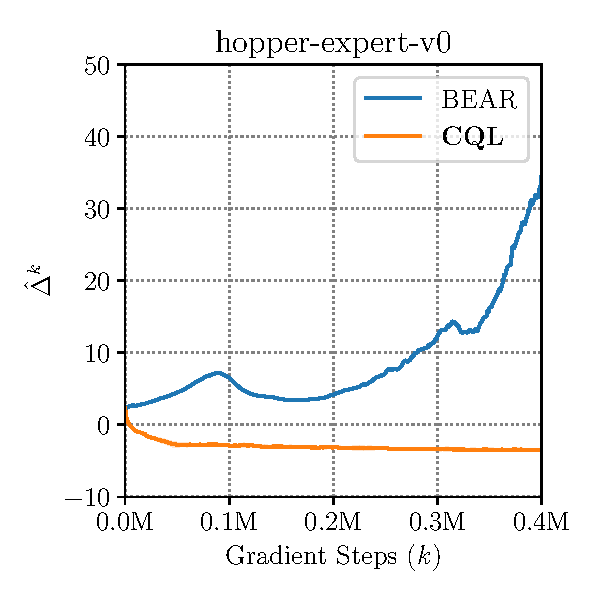
\includegraphics[width=0.47\linewidth]{chapters/cql/images/hopper-expert-v0bear_vs_cql.pdf}
      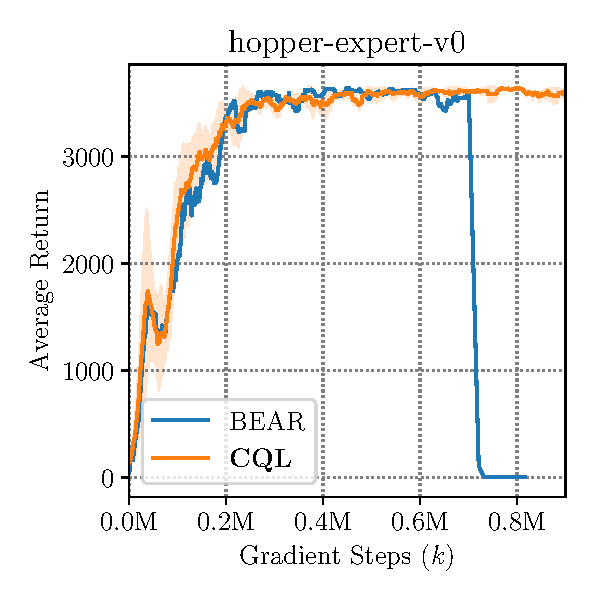
\includegraphics[width=0.47\linewidth]{chapters/cql/images/hopper-expert-v0bear_vs_cql_return.pdf}
      \caption{hopper-expert-v0}
    \end{subfigure}
    ~
    \begin{subfigure}[h]{0.49\linewidth}
      \centering
      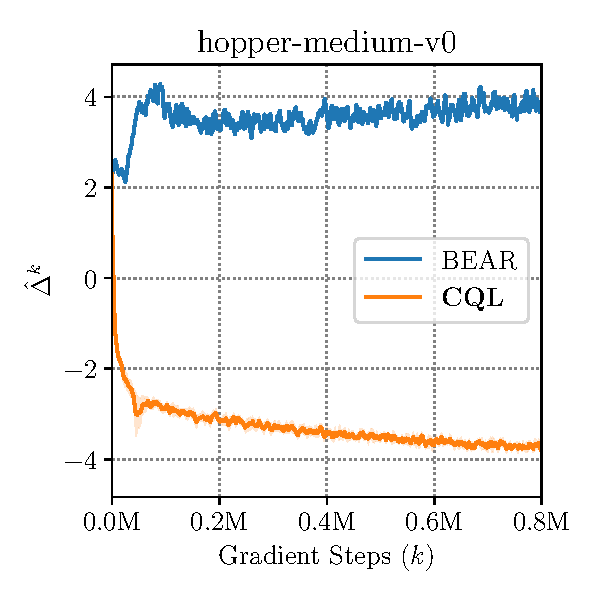
\includegraphics[width=0.47\linewidth]{chapters/cql/images/hopper-medium-v0bear_vs_cql_again.pdf}
      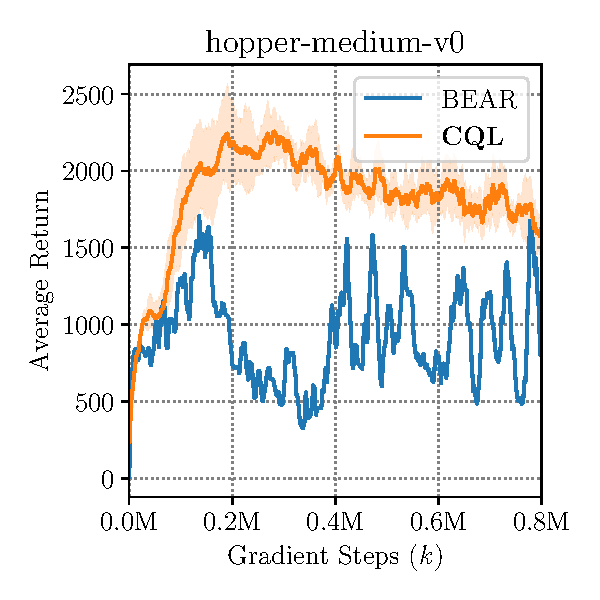
\includegraphics[width=0.47\linewidth]{chapters/cql/images/hopper-medium-v0bear_vs_cql_again_return.pdf}
      \caption{hopper-medium-v0}
      %%SL.5.27: label the plots -- label both axes and title
    \end{subfigure}
    \caption{$\Delta^k$ as a function of training iterations for hopper-expert and hopper-medium datasets. Note that CQL (left) generally has negative values of $\Delta$, whereas BEAR (right) generally has positive $\Delta$ values, which also increase during training with increasing $k$ values.}
    %%SL.5.27: Make sure caption at least briefly summarizes the implications of this
    \label{fig:delta_plots}
    \vspace{-0.2cm}
\end{figure}

% \textbf{Why does CQL solve this problem?} Theorem~\ref{thm:gap_amplify} indicates that, by appropriately controlling for $\alpha_k$, CQL can ensure that the learned $\hat{\Delta}^k$ is larger than the actual value of $\Delta^k$ in the MDP (when evaluated using the true Q-function, $Q^k$). That is, for all $k$, we have that $\hat{\Delta}^k > \Delta^k$ under appropriate choices of $\alpha_1, \cdots, \alpha_k$. Empirically, this translates to generally negative (or positive with a small magnitude) values of $\hat{\Delta}^k$ for CQL, as shown in Figure~\ref{fig:delta_plots}(a) and (b). Note that it is sufficient for the empirical $\hat{\Delta}^k$ to be larger than $\Delta^k$, and not necessarily negative. 
% %%AK.5.26: Revisit this statement once.
% CQL generally maintains a negative value of $\hat{\Delta}^k$, and this difference is reflected in better and more stable final policy performance for CQL, as shown in Figure ??, even without a policy constraint. 
